\section{Analysis}
\label{sec:analysis}

\subsection{Verifier Audit and Robustness}
\label{sec:verifier_audit}

\Cref{tab:verifier_audit} summarises verifier contradiction detection rates by claim
type under the \texttt{balanced} profile ($n{=}2000$, clean vs.\ 20\% noise
injection). Across 9{,}780 total claims, object existence is the strongest detection
family: 25.3\% on clean data (844/3{,}337), rising to 34.7\% under 20\% noise
injection (1{,}157/3{,}337). Attribute and spatial detection remain lower, reflecting
scene-graph annotation density (2.1\% and 4.5\% on clean, respectively).
Action claim detection is zero on clean data but rises sharply with injected noise
(20.2\% at 20\%), suggesting that action claims are structurally verifiable but
under-covered by the clean scene-graph oracle. OCR detection is effectively zero
across all noise levels---a known limitation of GQA scene graphs as a verification
oracle for text-in-image claims.

\begin{table}[h]
\centering
\caption{Verifier contradiction detection by claim type (\texttt{balanced}
profile, $n{=}2000$). Detection rates rise with injected noise; OCR is a known
gap. Claim counts reflect the $n{=}2000$ run (total: 9{,}780 claims).}
\label{tab:verifier_audit}
\small
\setlength{\tabcolsep}{3.5pt}
\begin{tabular}{lrrrr}
\toprule
\textbf{Claim Type} & \textbf{Count} & \textbf{Clean} & \textbf{Noise-0.1} & \textbf{Noise-0.2} \\
\midrule
Object Existence & 3{,}337 & 25.3\% & 29.5\% & 34.7\% \\
Attribute        & 2{,}913 &  2.1\% &  2.8\% &  3.8\% \\
Action           & 1{,}502 &  0.0\% & 11.1\% & 20.2\% \\
Spatial          & 1{,}604 &  4.2\% &  5.9\% &  7.2\% \\
Counting         &     24  & 54.2\% & 50.0\% & 50.0\% \\
OCR              &    400  &  0.0\% &  0.0\% &  0.0\% \\
\bottomrule
\end{tabular}
\end{table}

\begin{figure}[t]
  \centering
  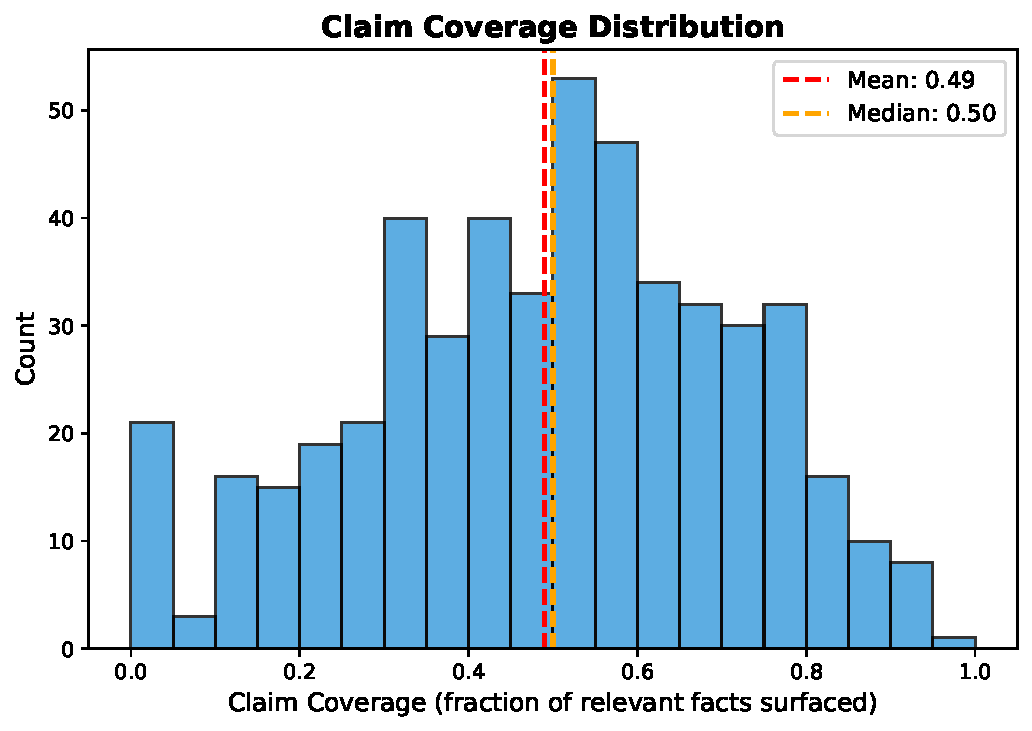
\includegraphics[width=0.85\linewidth]{figures/claim_coverage}
  \caption{Distribution of claim coverage over scene-graph facts
  (Qwen2.5-VL, $n{=}500$). Mean coverage is 0.49, meaning roughly half
  of all verifiable scene facts are surfaced as explicit beliefs per question.
  This low coverage implies that the 33.3\% premise-error rate is a
  conservative lower bound.}
  \label{fig:claim_coverage}
\end{figure}

\begin{figure}[t]
  \centering
  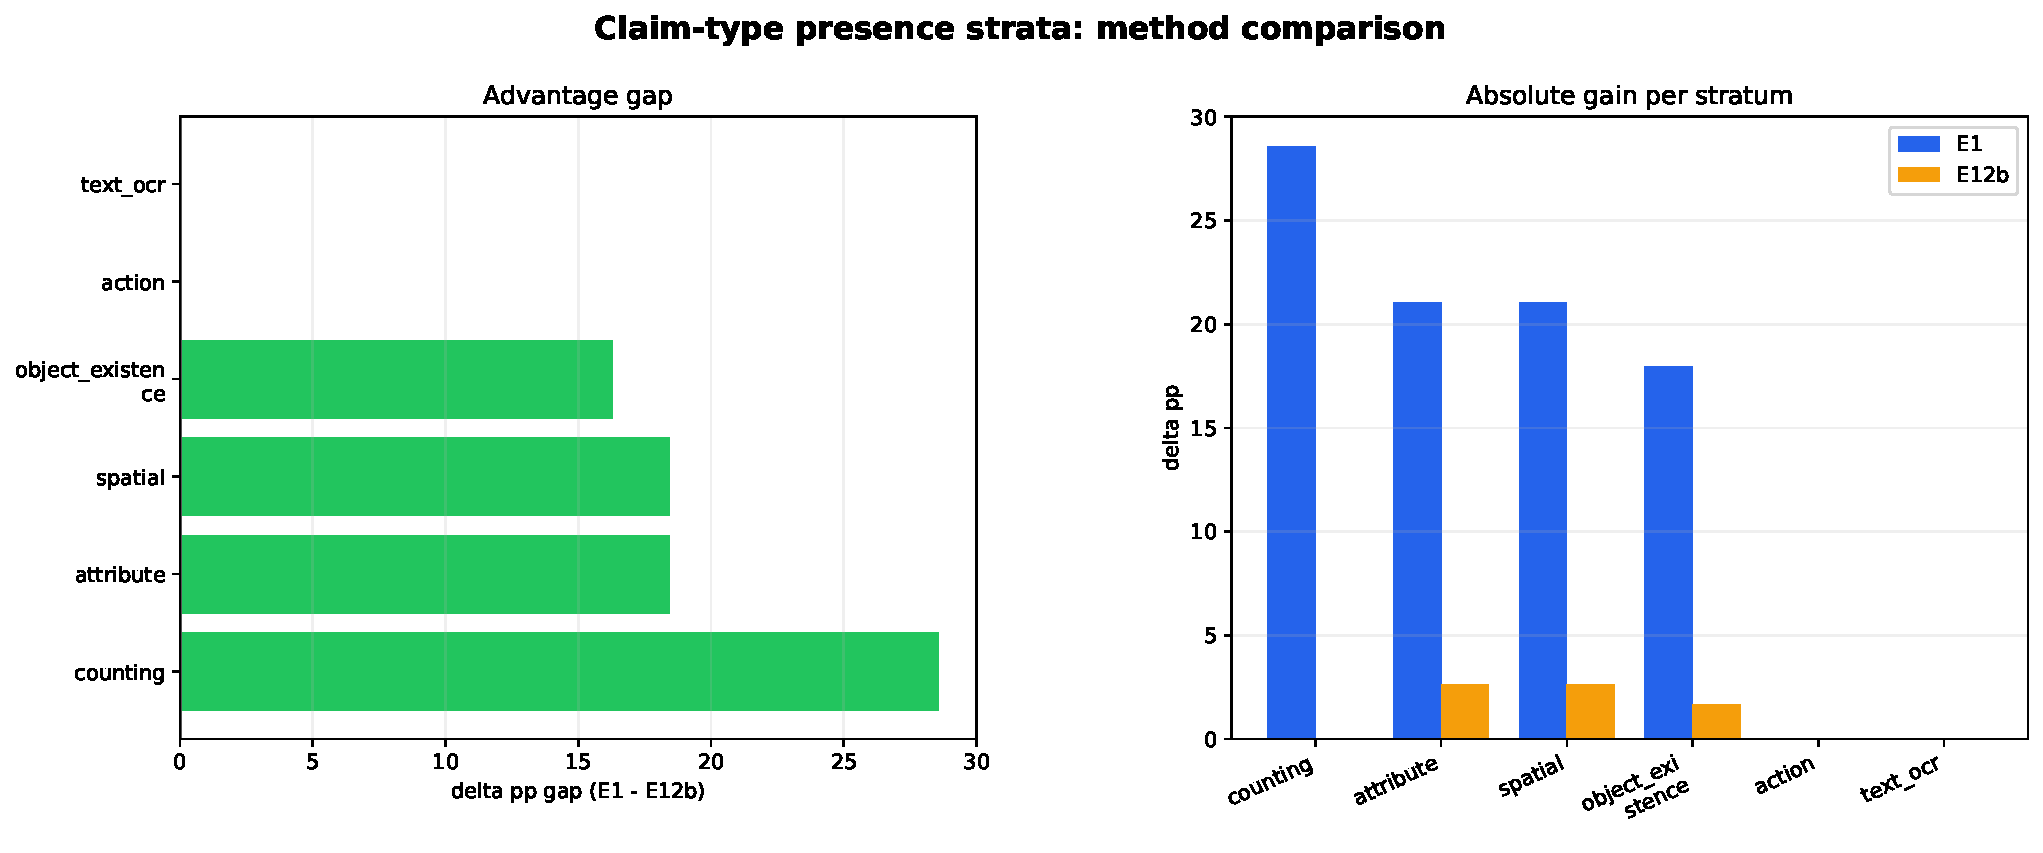
\includegraphics[width=\linewidth]{figures/task4_error_stratification_report_p4}
  \caption{Claim-type presence strata: E1 and E12b accuracy gain (pp) for
  samples containing each claim type. Counting ($+28.57$~pp E1 gap),
  attribute ($+18.42$~pp), and spatial ($+18.42$~pp) strata show the
  largest E1 advantage, while action and OCR strata are zero due to
  verifier coverage gaps on these claim families.}
  \label{fig:claim_strata}
\end{figure}

\begin{figure}[t]
  \centering
  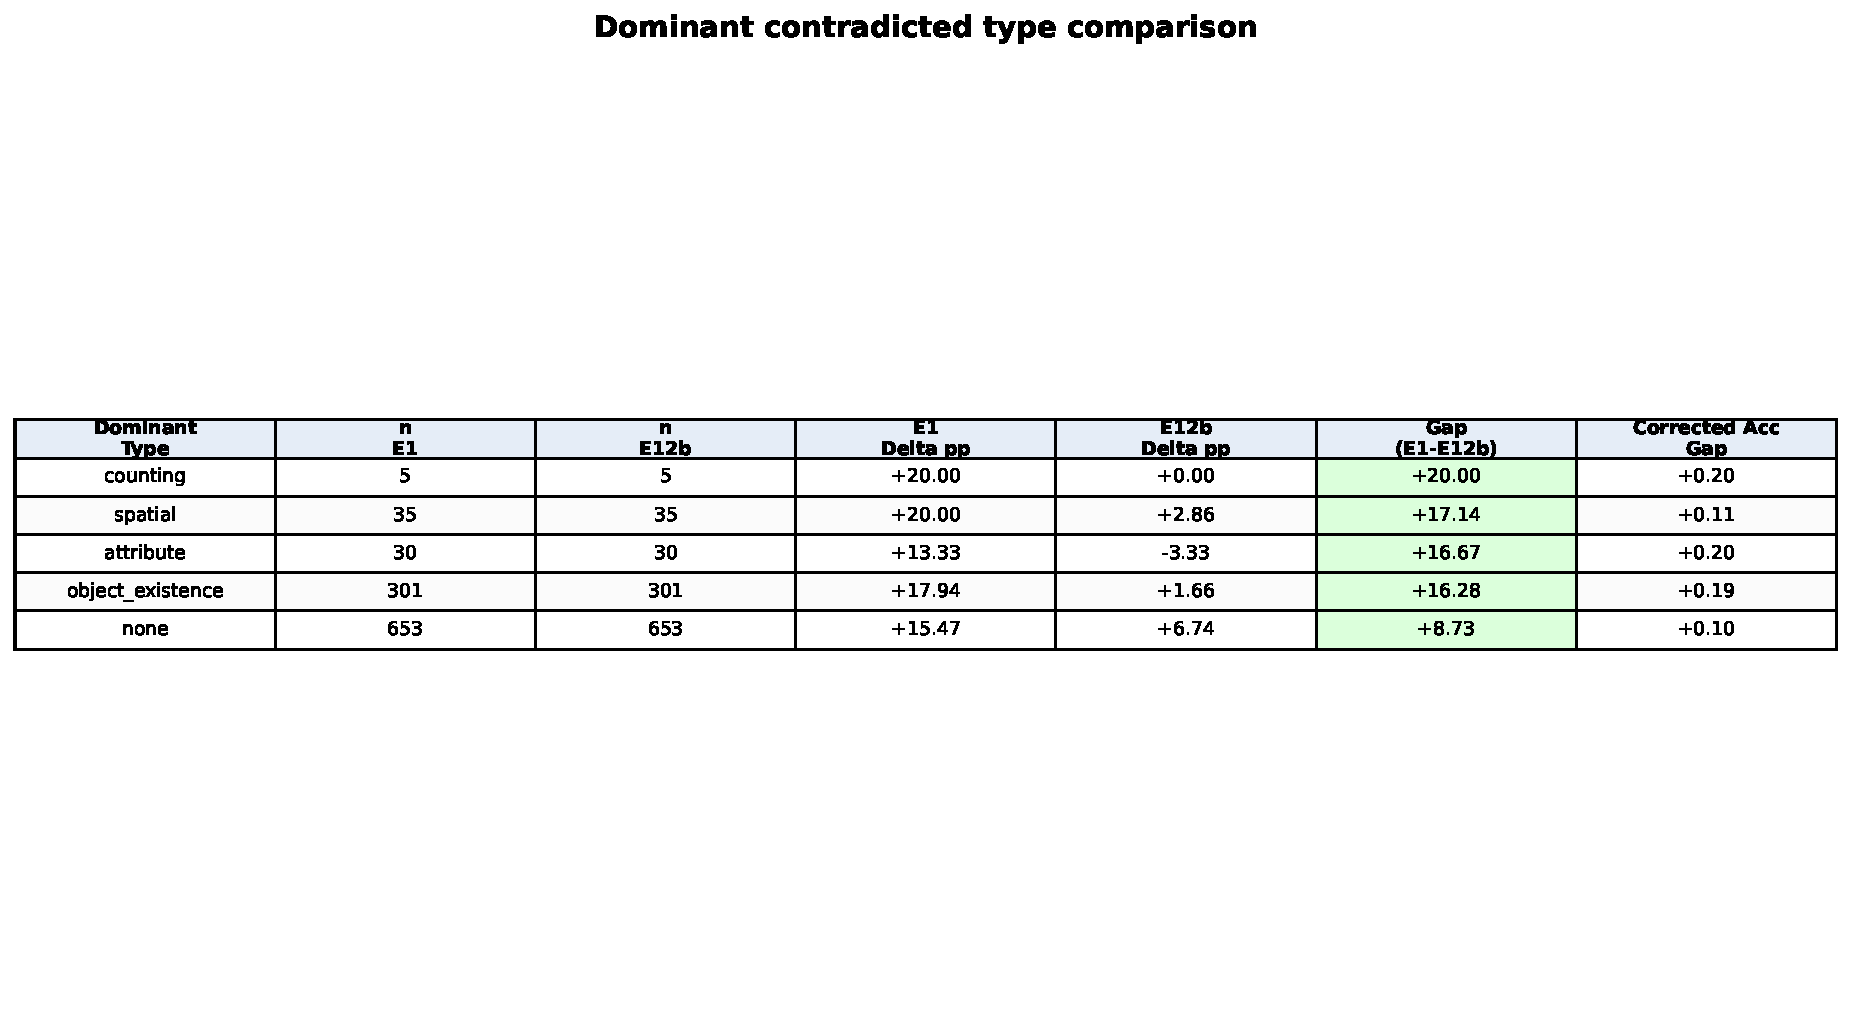
\includegraphics[width=\linewidth]{figures/task4_error_stratification_report_p5}
  \caption{Dominant contradicted claim type comparison (E1 vs.\ E12b, $n{=}500$
  subset). When counting or spatial claims dominate the contradiction profile,
  E1 outperforms E12b by $+17$--$20$~pp. Object-existence-dominated samples
  show a $+16.28$~pp gap. Even samples with no detectable contradiction
  (``none'') benefit from E1 ($+15.47$~pp), likely via implicit false beliefs
  missed by the verifier.}
  \label{fig:dominant_claim_type}
\end{figure}

Profile comparison (\texttt{strict} vs.\ \texttt{balanced} vs.\ \texttt{high\_recall})
at $n{=}2000$ shows near-identical behavior on clean object detection (all 25.3\%),
diverging primarily on spatial and action categories under noise. This confirms that
the \texttt{balanced} profile is a reliable default and that the 33.3\% premise-error
rate is robust to moderate verifier configuration choices.

These results have two implications for interpreting the main findings.
First, the 33.3\% premise-error rate is a conservative lower bound due to missed
detections in attribute and action categories.
Second, the verifier degrades gracefully under moderate noise (5--10\%), supporting
robustness of the pipeline to annotation imperfection.

\subsection{Belief Externalization Quality}
\label{sec:belief_quality}

\Cref{tab:model_compare} compares LLaVA-1.5-7B~\cite{liu2023visual} and
Qwen2.5-VL-7B~\cite{bai2025qwen} on belief quality and downstream premise-error
observability. Qwen produces $2.3{\times}$ more beliefs per question on average
(4.96 vs.\ 2.17) and achieves 14.5~pp higher baseline accuracy (59.2\% vs.\ 52.2\%).
Crucially, Qwen's richer belief sets yield nearly double the observed premise-error
rate (33.3\% vs.\ 18.8\%), suggesting that sparse or over-hedged beliefs suppress
the observable PE rate even when premise errors are present.
Our results indicate that belief externalization quality is a critical design variable:
models that emit vague or entity-level beliefs rather than typed, grounded predicates
limit the effectiveness of the verification stage.

\begin{table}[h]
\centering
\caption{Model comparison on GQA ($n{=}500$). Richer belief externalization
yields higher observed premise-error rates and better base accuracy.}
\label{tab:model_compare}
\small
\setlength{\tabcolsep}{4pt}
\begin{tabular}{lcccc}
\toprule
\textbf{Model} & \textbf{Acc.} & \textbf{PE Rate} & \textbf{RE Rate}
  & \textbf{Avg.\ Beliefs} \\
\midrule
LLaVA-1.5-7B  & 52.2\% & 18.8\% & 81.2\% & 2.17 \\
Qwen2.5-VL-7B & 59.2\% & 33.3\% & 66.7\% & 4.96 \\
\bottomrule
\end{tabular}
\end{table}

\subsection{Belief Minimality}

In 27.9\% of premise-error cases (19/68), removing or replacing a \emph{single}
contradicted belief is sufficient to flip the answer to correct
(see \cref{fig:belief_minimality}). This single-belief
minimality rate reveals that many failures are sensitive to one false premise.
The remaining 72.1\% of cases likely involve multiple interacting false premises,
motivating the full replacement strategy of E1 over the single-removal E3 policy.
The minimality result also suggests that a future ranking of beliefs by confidence
could yield efficient, surgical interventions without requiring access to full
ground-truth scene graphs.

\begin{figure}[t]
  \centering
  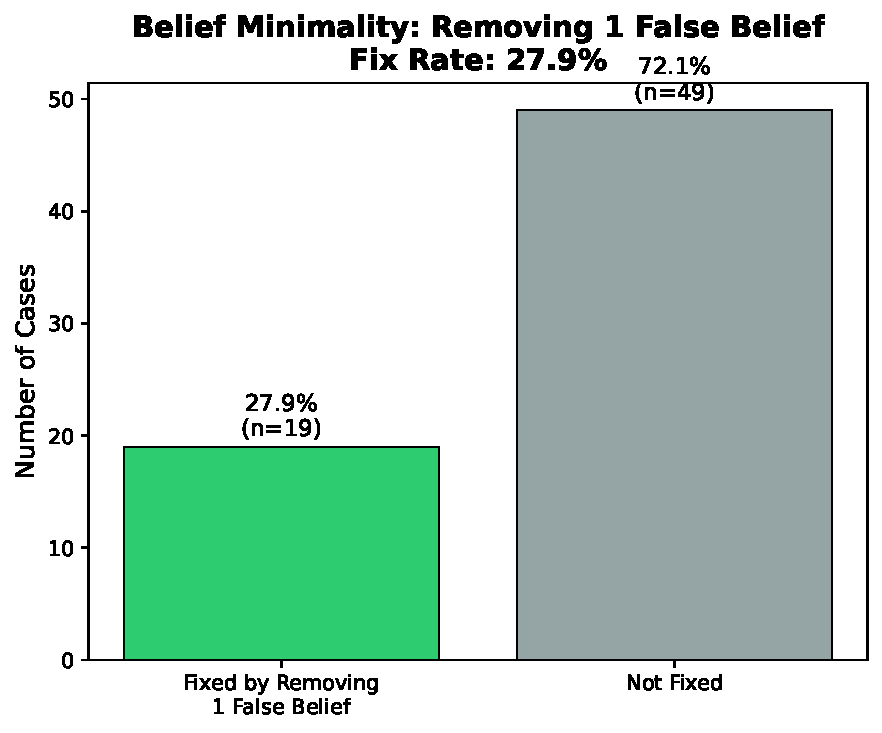
\includegraphics[width=0.75\linewidth]{figures/belief_minimality}
  \caption{Belief minimality among premise-error cases ($n{=}68$).
  In 27.9\% of cases (19/68), removing a \emph{single} contradicted belief
  suffices to flip the answer to correct, revealing high sensitivity to
  individual false premises. The remaining 72.1\% involve multiple
  interacting errors, motivating the full replacement strategy of E1.}
  \label{fig:belief_minimality}
\end{figure}

\subsection{Confidence-Gated Policy Analysis (E12b)}
\label{sec:e12b_analysis}

E12b applies correction only when the intervention score $s \geq \tau{=}0.18$.
This threshold was selected via a paired comparison against the stricter E12 variant
($\tau{=}0.25$): lowering the threshold from 0.25 to 0.18 increased the intervention
rate from 35.2\% to 58.8\%, yielding 25 additional wins at a cost of only 11 losses
(McNemar $p{=}0.0288$, net $+14$ samples corrected; E12: 59.6\%; E12b: 62.4\%).

At $n{=}2000$, E12b achieves an intervention rate of 59.85\% with a near-zero
fallback rate of 0.10\%. The resulting $+3.45$~pp gain shows that selective
correction at roughly 60\% coverage captures most of the recoverable gain under
practical compute constraints. Multi-seed stability (seeds 42, 123, 456) yields
$66.18\% \pm 0.14$~pp, confirming numerical robustness across random subsamples.

\subsection{Threshold Robustness of E12b}
\label{sec:threshold_robustness}

To verify that $\tau{=}0.18$ is not a fragile optimum, we sweep five thresholds
$\tau \in \{0.10, 0.14, 0.18, 0.22, 0.26\}$ on a held-out seed ($n{=}500$, seed 123)
and report accuracy gain, intervention rate, and net gain rate.

\Cref{fig:threshold_acc,fig:threshold_rates} show that all five thresholds produce
positive gains over the baseline (60.6\%), and the intervention rate decreases
monotonically with $\tau$ (verified: zero monotonicity violations).
Lower thresholds intervene on more samples (78\% at $\tau{=}0.10$ vs.\
34\% at $\tau{=}0.26$) and yield larger absolute gains ($+2.0$~pp vs.\ $+0.4$~pp),
confirming the expected coverage/precision trade-off.

Crucially, no threshold \emph{hurts} performance: even the most conservative setting
($\tau{=}0.26$) still improves accuracy by $+0.4$~pp. McNemar tests of each threshold
against the anchor $\tau{=}0.18$ show no significant difference ($p > 0.4$ for all),
confirming that performance is insensitive to moderate threshold variation and that
$\tau{=}0.18$ is a robust operating point.

\begin{figure}[t]
  \centering
  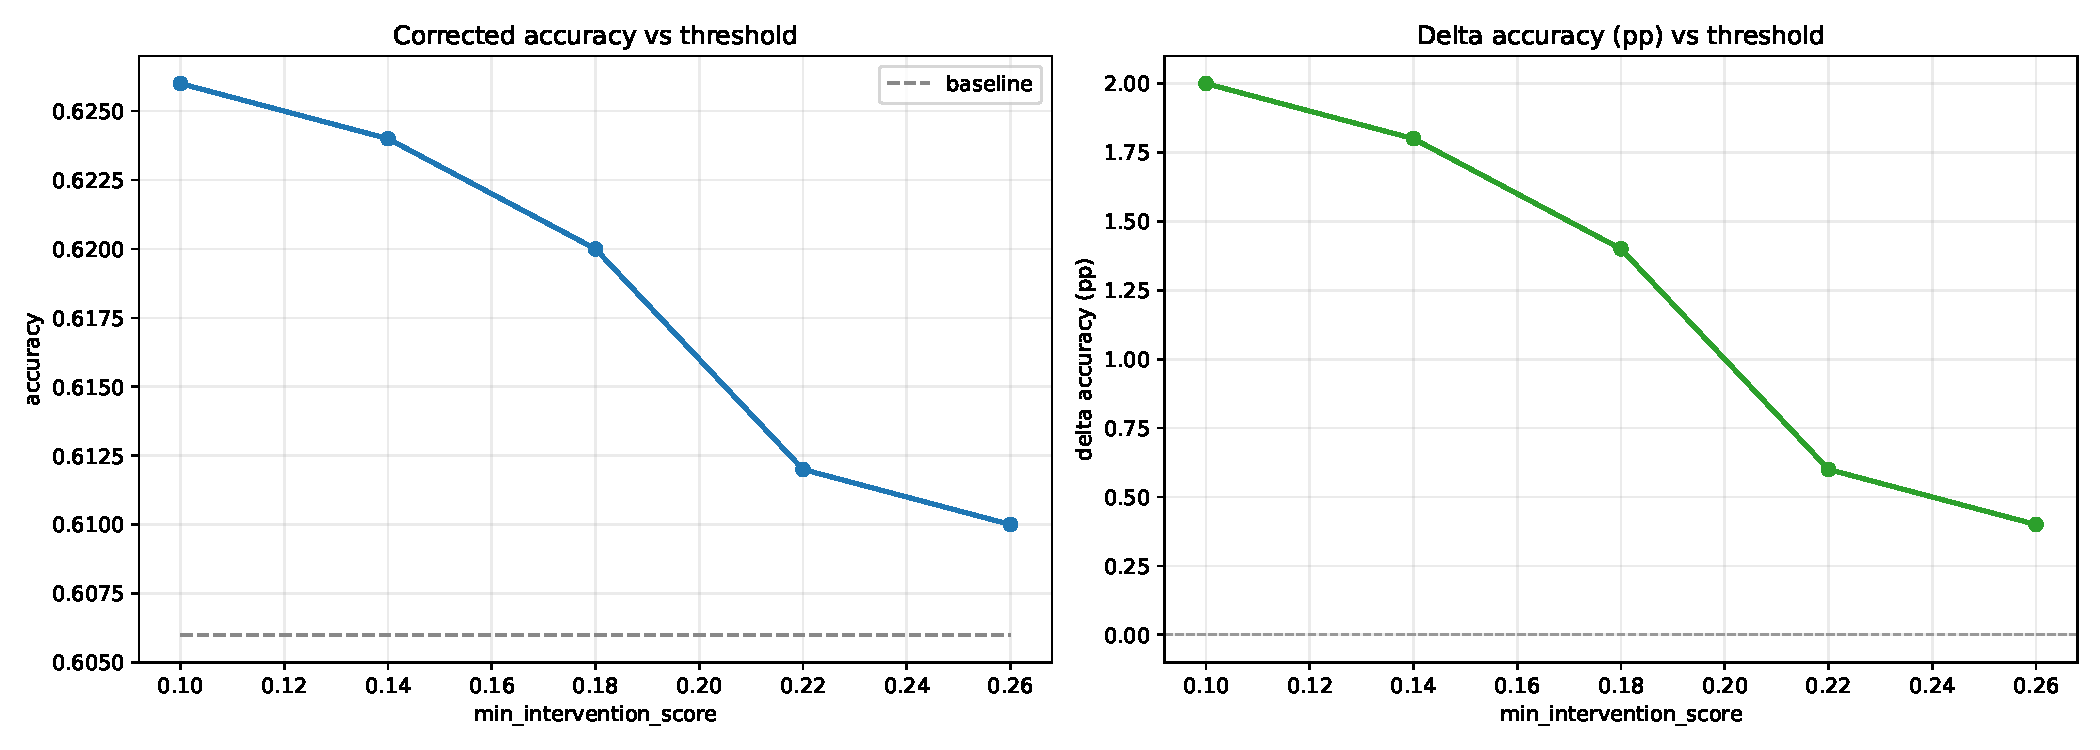
\includegraphics[width=\linewidth]{figures/task6_threshold_robustness_report_p1}
  \caption{Threshold sweep for E12b ($n{=}500$, seed 123).
  Left: corrected accuracy vs.\ $\tau$ --- all thresholds exceed the baseline
  (dashed, 60.6\%), with gains decreasing monotonically from $+2.0$~pp at
  $\tau{=}0.10$ to $+0.4$~pp at $\tau{=}0.26$.
  Right: accuracy gain (pp) vs.\ $\tau$. No threshold hurts performance.}
  \label{fig:threshold_acc}
\end{figure}

\begin{figure}[t]
  \centering
  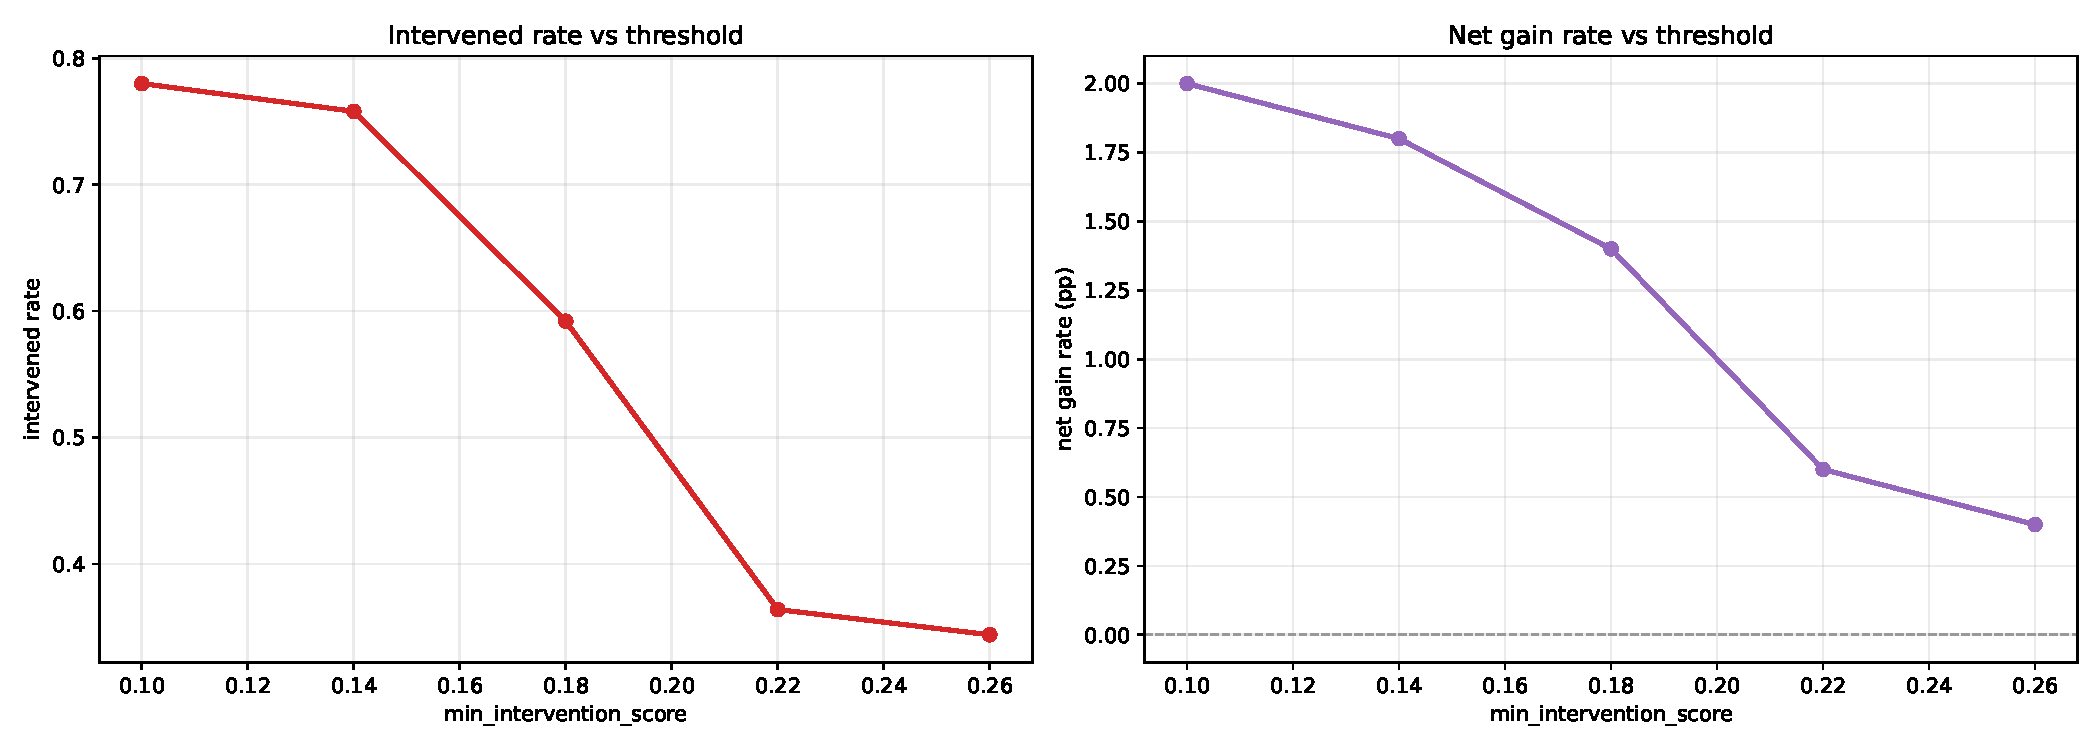
\includegraphics[width=\linewidth]{figures/task6_threshold_robustness_report_p2}
  \caption{Intervention rate (left) and net gain rate (right) vs.\ threshold $\tau$.
  Both decrease monotonically: intervention rate falls from 78\% at $\tau{=}0.10$
  to 34\% at $\tau{=}0.26$; net gain rate from 2.0 to 0.4~pp. The strict
  monotonicity (zero violations) confirms the score is a reliable proxy for
  intervention quality.}
  \label{fig:threshold_rates}
\end{figure}

\begin{figure}[t]
  \centering
  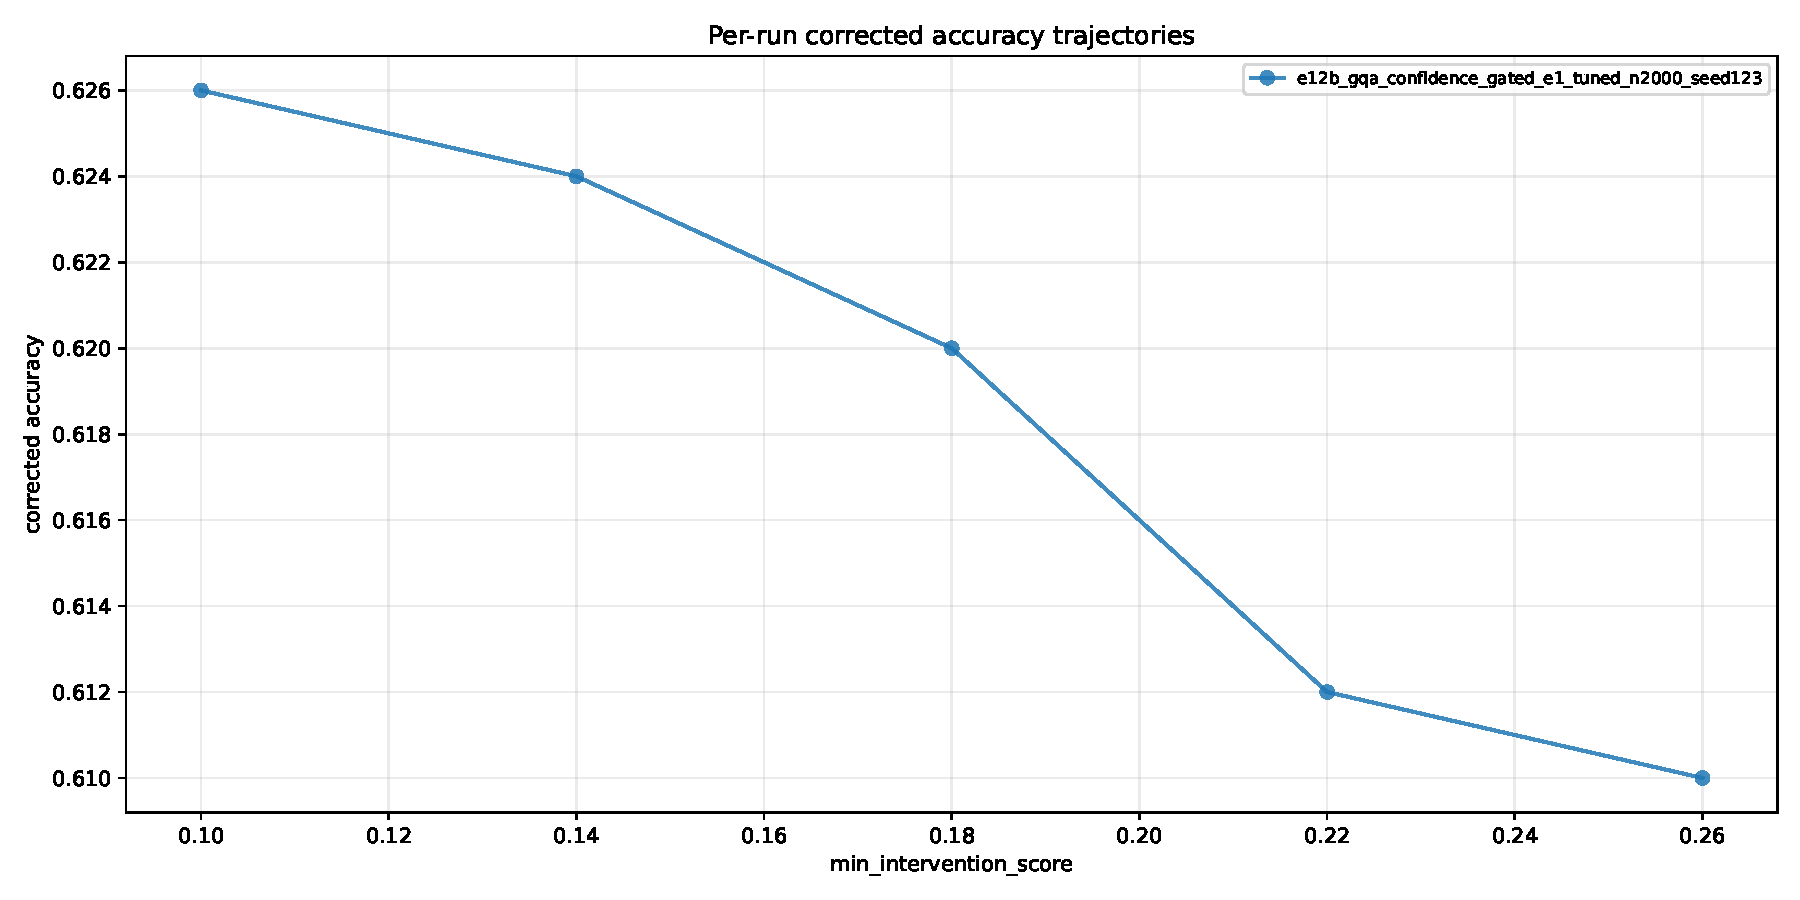
\includegraphics[width=0.75\linewidth]{figures/task6_threshold_robustness_report_p3}
  \caption{Per-run corrected accuracy trajectory across all five $\tau$ values
  (seed 123). The smooth, strictly monotone-decreasing curve confirms that
  score-based gating behaves predictably: tighter gates yield lower but never
  negative gains. The $\tau{=}0.18$ operating point (middle) provides the
  best balance between coverage and per-intervention reliability.}
  \label{fig:threshold_trajectory}
\end{figure}

\subsection{Cost-Efficiency}
\label{sec:cost}

\Cref{tab:cost} compares E1 and E12b at $n{=}2000$ on wall-clock efficiency.
E1 achieves $+16.2$~pp in 15{,}629\,s ($\approx$7.81\,s/sample), while E12b
achieves $+3.45$~pp in 15{,}980\,s ($\approx$7.99\,s/sample). The gain-per-unit-time
ratio strongly favors E1 when accuracy maximization is the goal (2.07 vs.\
0.43~pp per second per sample). E12b is preferred when compute is constrained but
a significant and reliable improvement is still desired.

\begin{table}[h]
\centering
\caption{Cost-efficiency comparison at $n{=}2000$.
E1 is superior when compute is unconstrained; E12b provides a practical alternative.}
\label{tab:cost}
\small
\setlength{\tabcolsep}{4pt}
\begin{tabular}{lrrrr}
\toprule
\textbf{Method} & \textbf{s/sample} & \textbf{Base Acc.} & \textbf{$\Delta$ pp} & \textbf{$\Delta$/s} \\
\midrule
E1 (n=2000)   & 7.81 & 63.55\% & $+16.2$ & 2.07 \\
E12b (n=2000) & 7.99 & 62.90\% & $+3.45$ & 0.43 \\
\bottomrule
\end{tabular}
\end{table}

\Cref{fig:cost_summary,fig:cost_pareto,fig:cost_gpu_hour,fig:cost_perrun} provide
a comprehensive cost-efficiency characterization across all runs.

\begin{figure}[t]
  \centering
  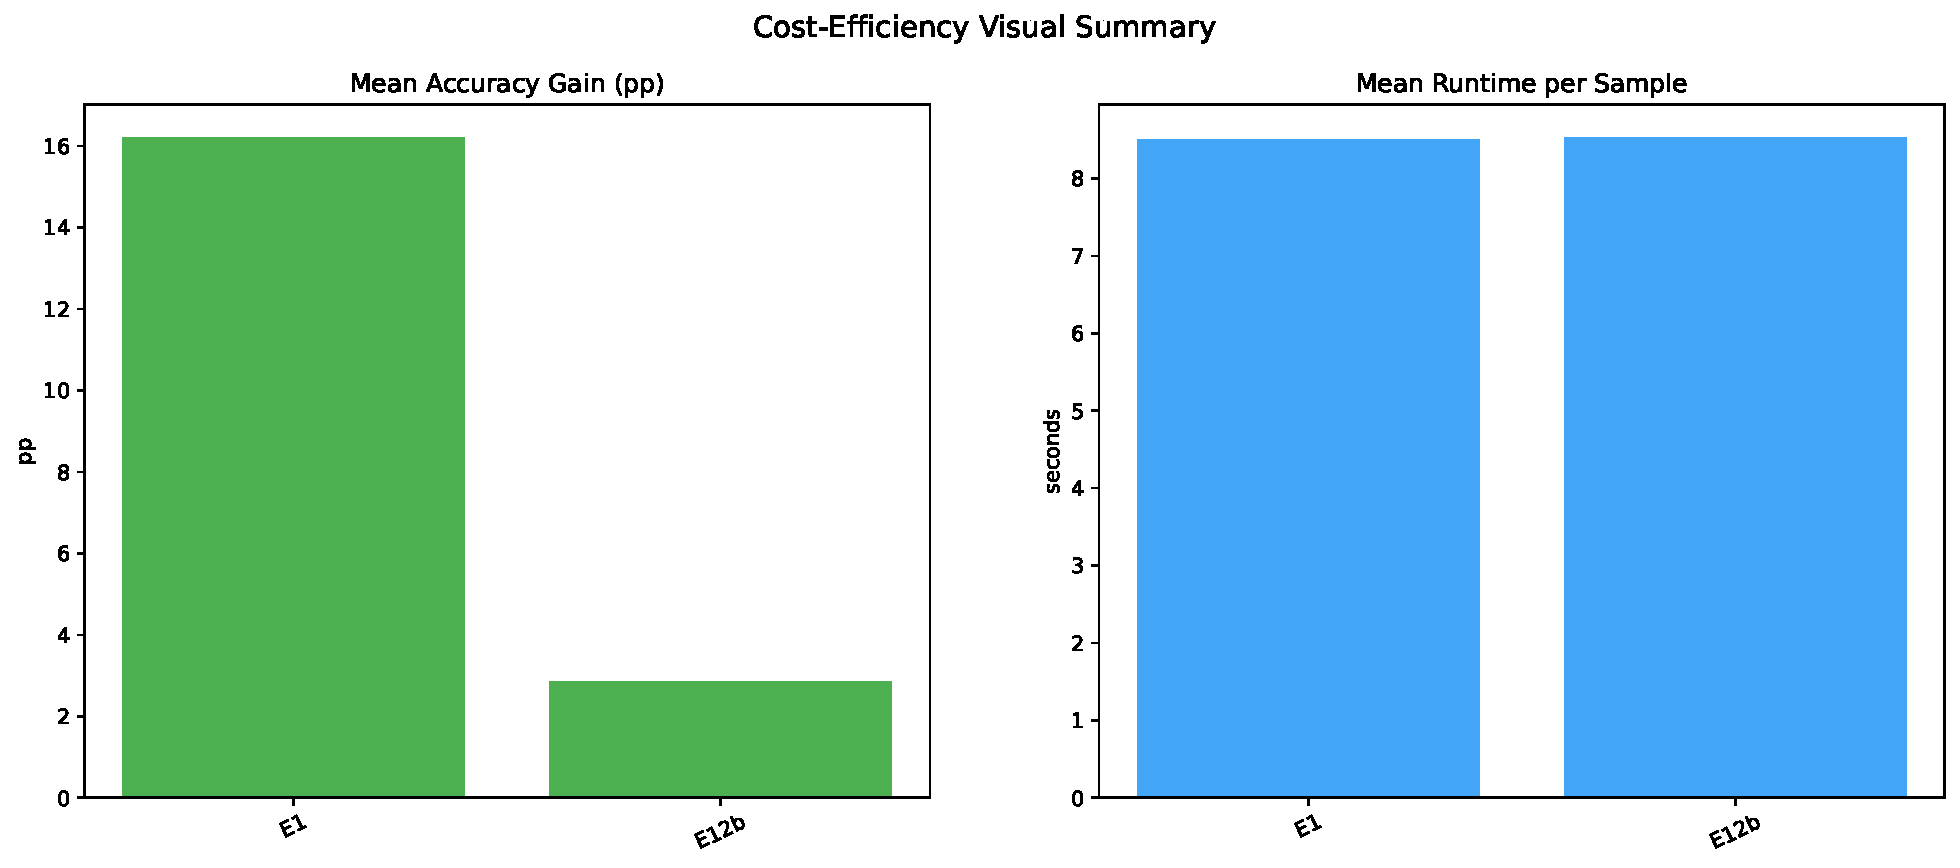
\includegraphics[width=\linewidth]{figures/cost_efficiency_report_p2}
  \caption{Cost-efficiency visual summary: mean accuracy gain (pp, left) and
  mean runtime per sample (seconds, right) for E1 and E12b across all runs.
  E1 achieves $5.8{\times}$ higher mean gain ($16.2$ vs.\ $2.85$~pp) at
  essentially identical per-sample cost ($8.50$ vs.\ $8.53$\,s/sample).}
  \label{fig:cost_summary}
\end{figure}

\begin{figure}[t]
  \centering
  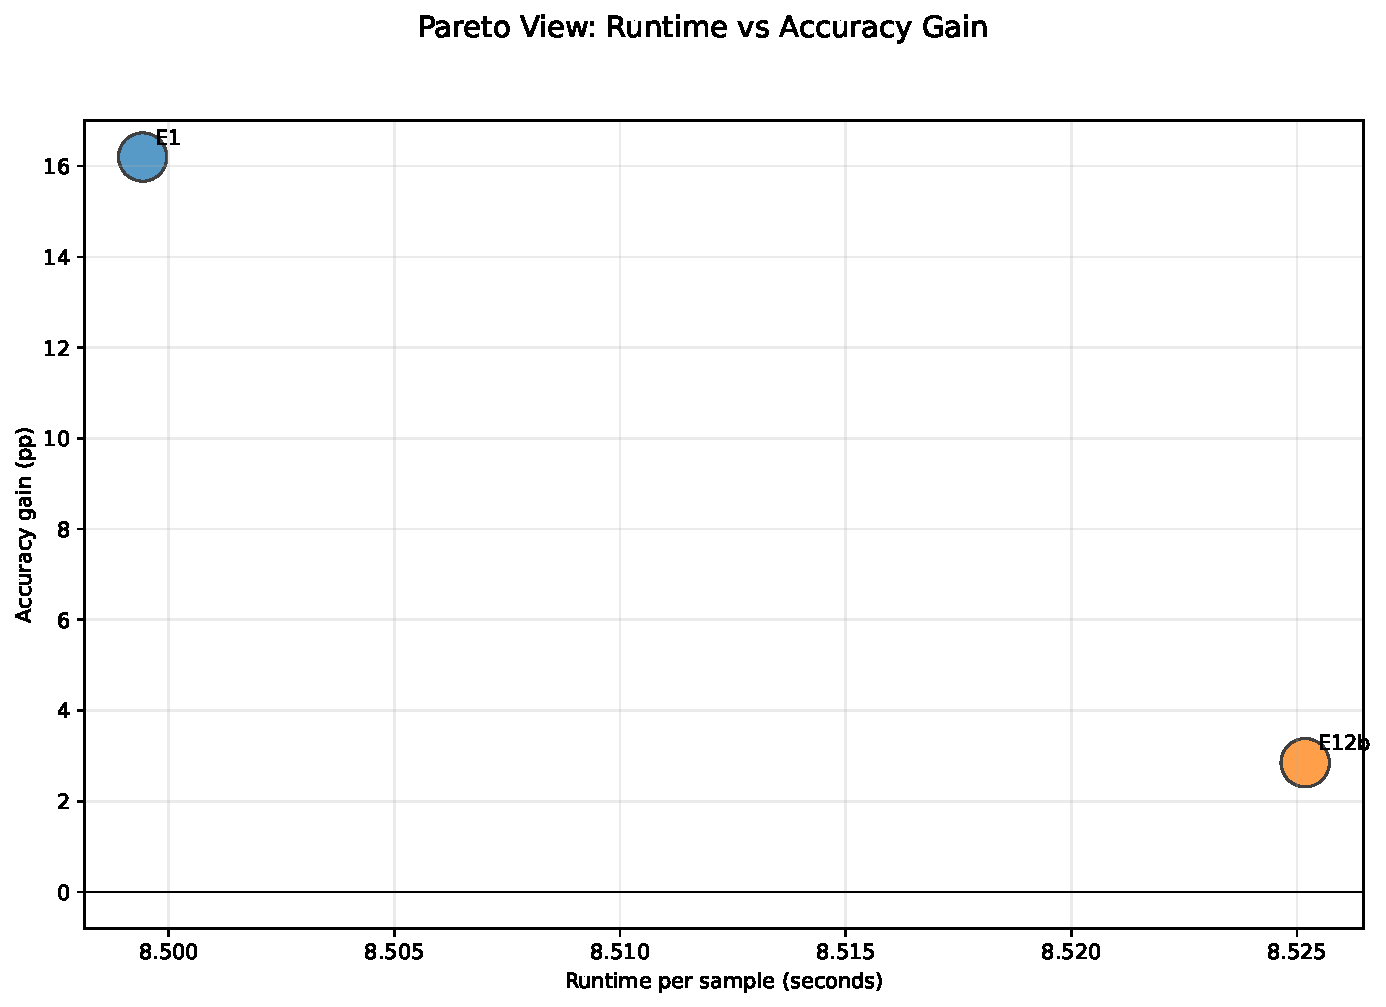
\includegraphics[width=0.75\linewidth]{figures/cost_efficiency_report_p3}
  \caption{Pareto view: runtime per sample vs.\ accuracy gain. E1 occupies
  the dominant position (top-left), achieving $+16.2$~pp at $8.50$\,s/sample.
  E12b offers a useful fallback at $+2.85$~pp for lower-certainty deployments.}
  \label{fig:cost_pareto}
\end{figure}

\begin{figure}[t]
  \centering
  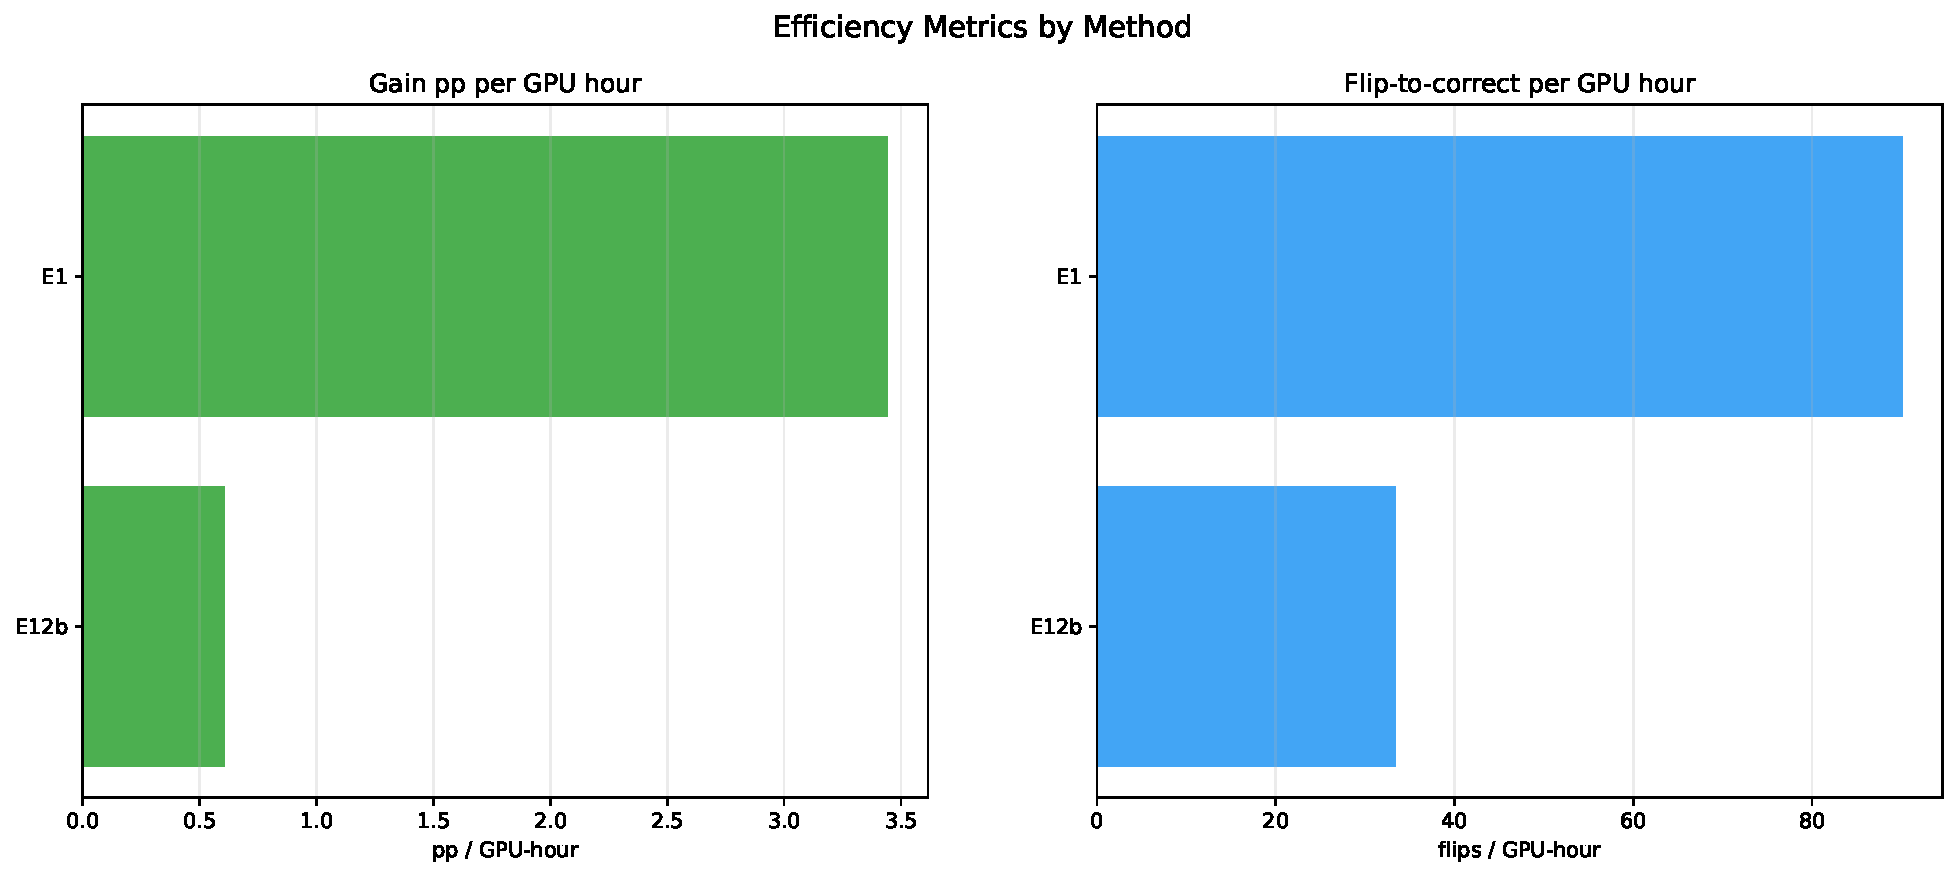
\includegraphics[width=\linewidth]{figures/cost_efficiency_report_p4}
  \caption{GPU-hour efficiency: gain pp/GPU-hour (left) and flips/GPU-hour
  (right). E1 achieves $3.44$~pp/GPU-hour and 90~flips/GPU-hour vs.\
  E12b at $0.61$~pp/GPU-hour and 33~flips/GPU-hour, confirming E1's
  dominance when accuracy per unit compute is the objective.}
  \label{fig:cost_gpu_hour}
\end{figure}

\begin{figure}[t]
  \centering
  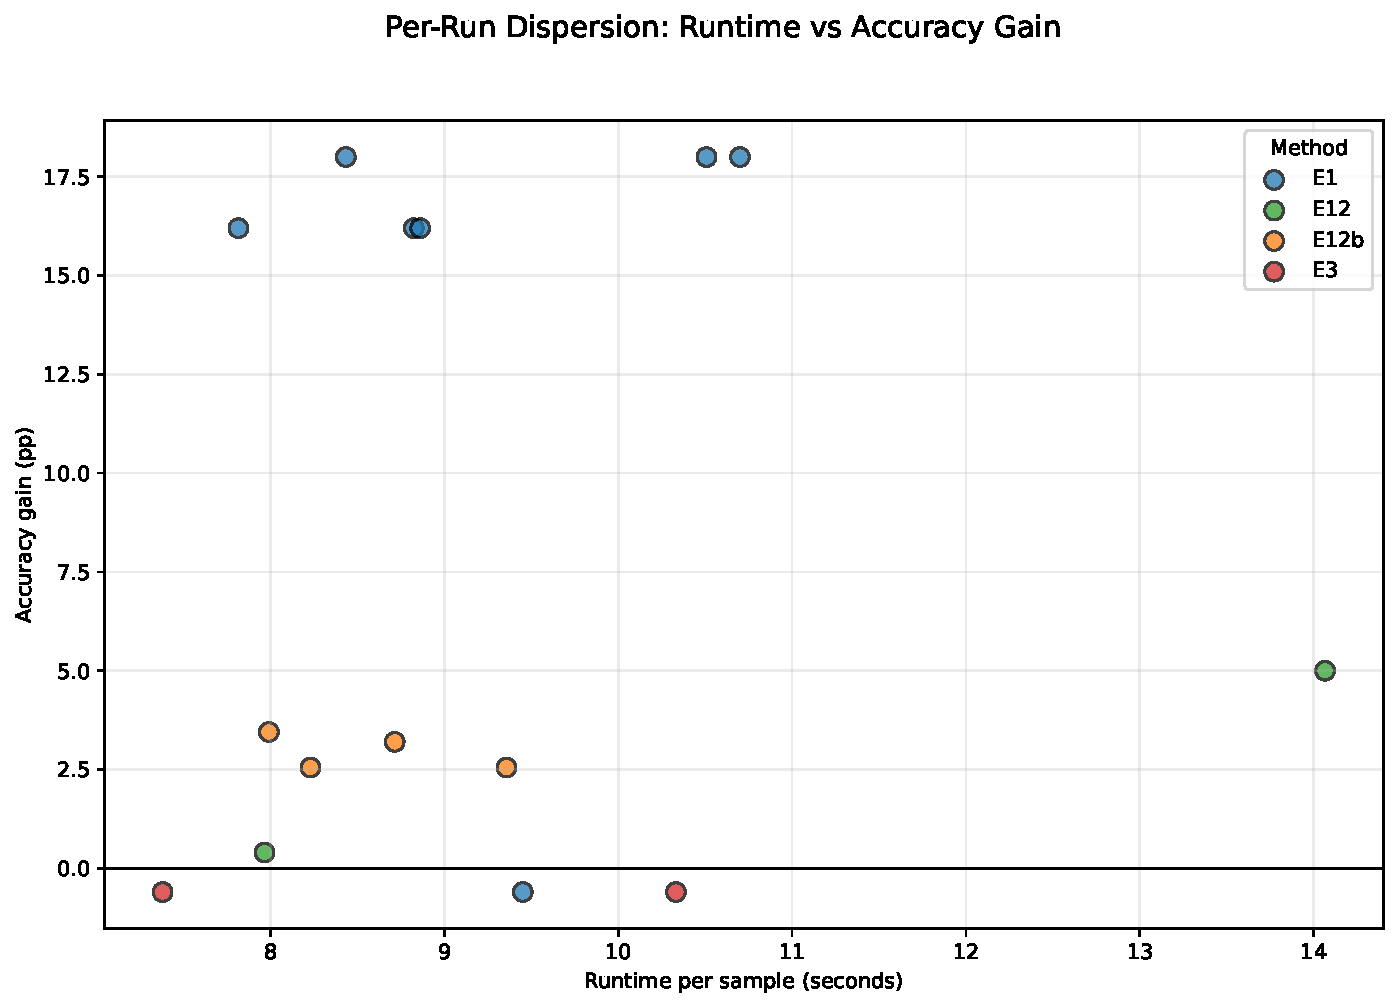
\includegraphics[width=\linewidth]{figures/cost_efficiency_report_p6}
  \caption{Per-run dispersion: runtime vs.\ accuracy gain across all 18
  individual runs (E1 blue, E12b orange, E12 green, E3 red). E1 runs
  cluster at $+16$--$18$~pp gain with $7.8$--$10.7$\,s/sample;
  E12b clusters at $+2.5$--$3.5$~pp; E3 runs show near-zero or negative
  gain, confirming that removal-only is not a viable policy.}
  \label{fig:cost_perrun}
\end{figure}

\subsection{Confidence Calibration and Abstention}
\label{sec:calibration}

We evaluate how well the intervention score $s$ is calibrated against the
observed corrected error rate, and whether score-based abstention can be used
to operate \bci{} at different coverage/accuracy trade-offs.

\paragraph{Calibration.}
E1 achieves ECE $= 0.0793 \pm 0.0000$ across three seeds, indicating strong
alignment between intervention score and error rate (\cref{fig:calib_reliability}).
E12b has higher ECE $= 0.1413 \pm 0.0007$, reflecting its conditional
intervention policy which skews the score distribution toward higher-confidence
corrections.

\begin{figure}[t]
  \centering
  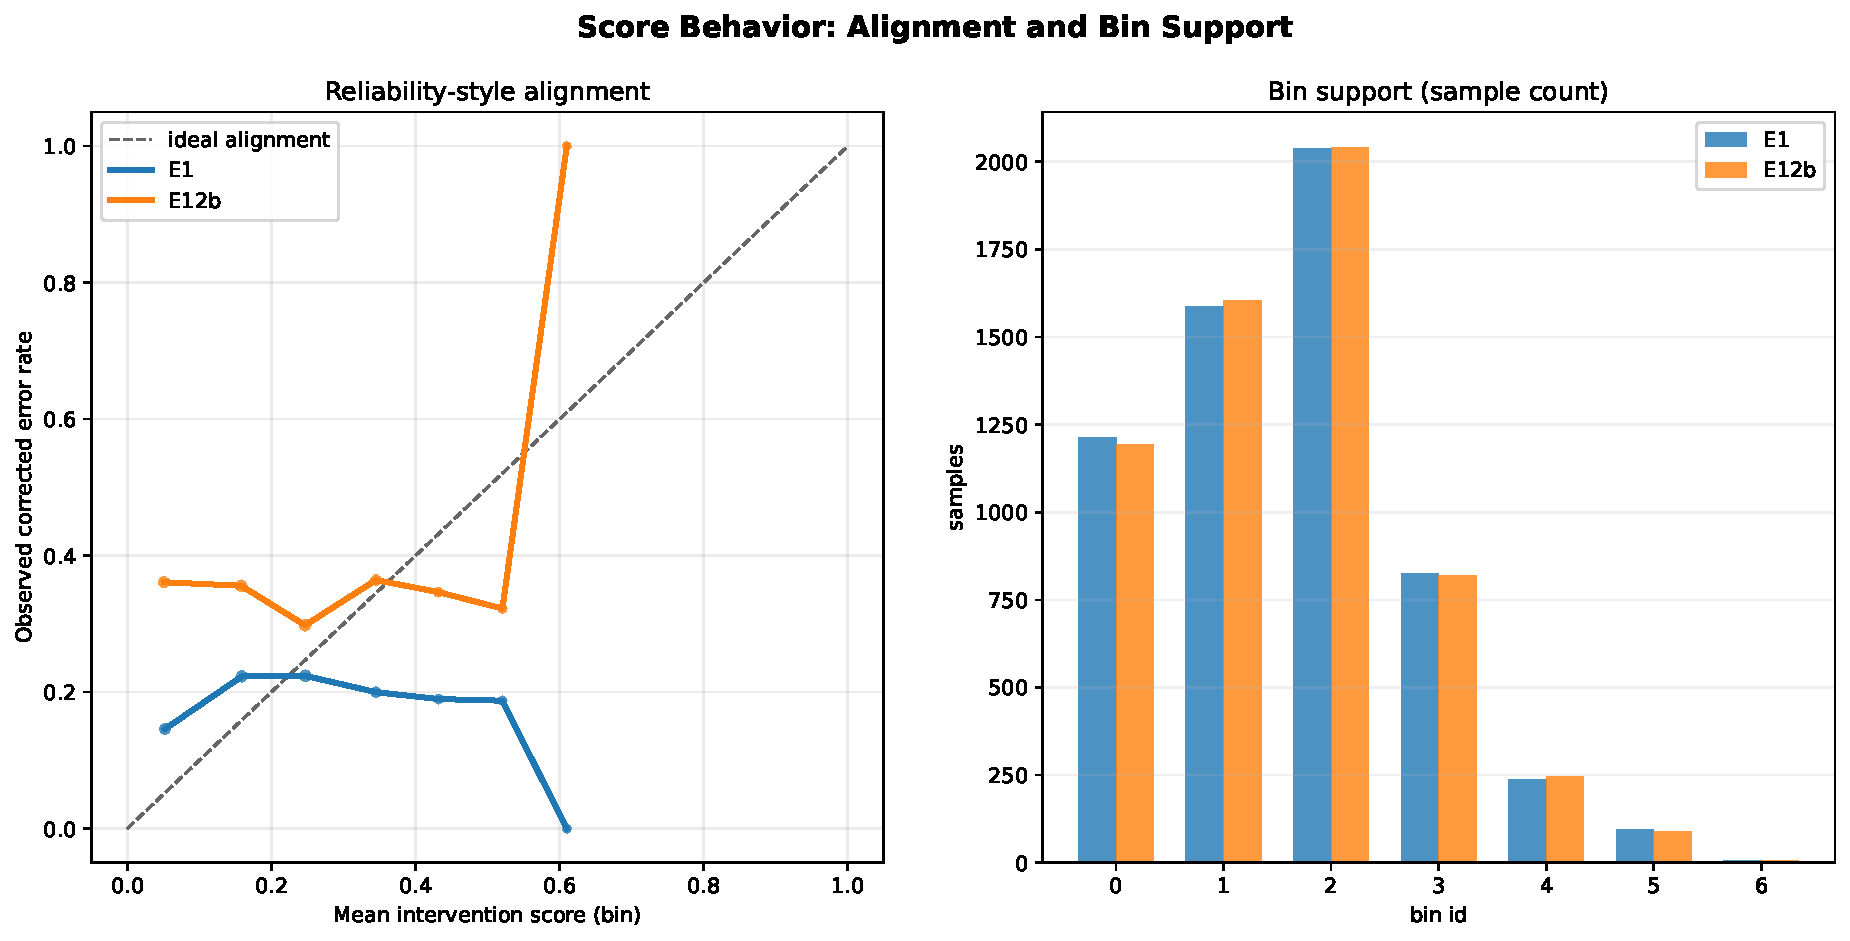
\includegraphics[width=\linewidth]{figures/task7_calibration_report_p2}
  \caption{Reliability diagram and bin support for E1 (blue) and E12b (orange).
  Left: E1 tracks the ideal diagonal closely (ECE$=0.079$); E12b deviates more
  at high scores (ECE$=0.141$). Right: bin support shows most samples fall in
  score bins 1--2 ($s \in [0.1, 0.3]$), indicating the majority of interventions
  operate in a well-calibrated mid-confidence regime.}
  \label{fig:calib_reliability}
\end{figure}

\begin{figure}[t]
  \centering
  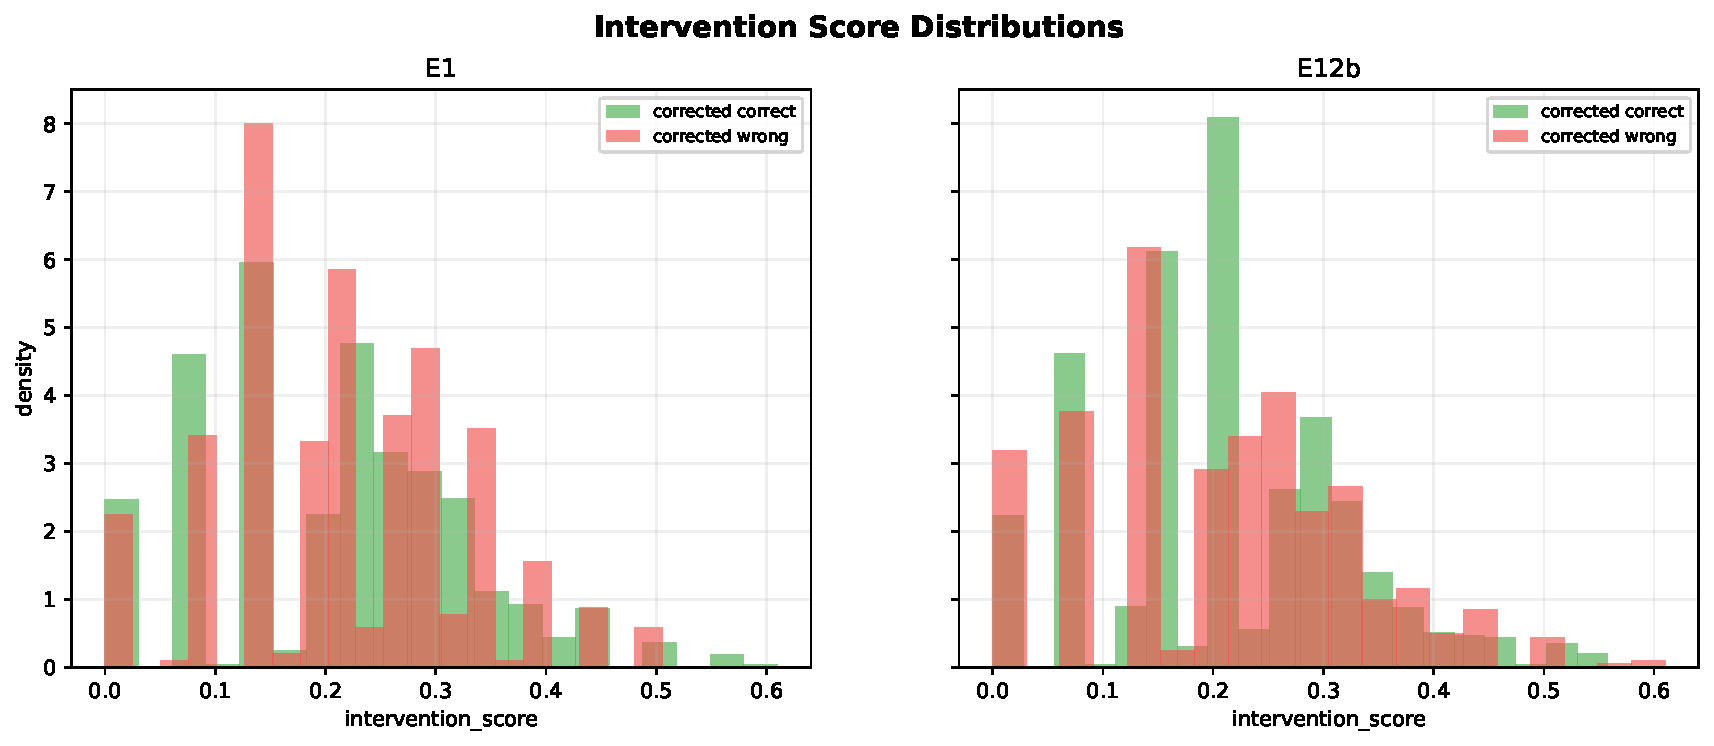
\includegraphics[width=\linewidth]{figures/task7_calibration_report_p3}
  \caption{Intervention score distributions for E1 (left) and E12b (right),
  stratified by outcome (corrected-correct: green; corrected-wrong: red).
  E1 shows substantial overlap between distributions, reflecting its
  unconditional policy. E12b's gating concentrates corrections in the
  $s \in [0.15, 0.30]$ range where green outcomes dominate.}
  \label{fig:calib_score_dist}
\end{figure}

\paragraph{Abstention.}
\Cref{fig:abstention_tradeoff,fig:abstention_gain,fig:abstention_oppoints}
characterize the coverage/accuracy trade-off under score-based abstention
(i.e., abstain on samples where $s$ exceeds a threshold).

\begin{figure}[t]
  \centering
  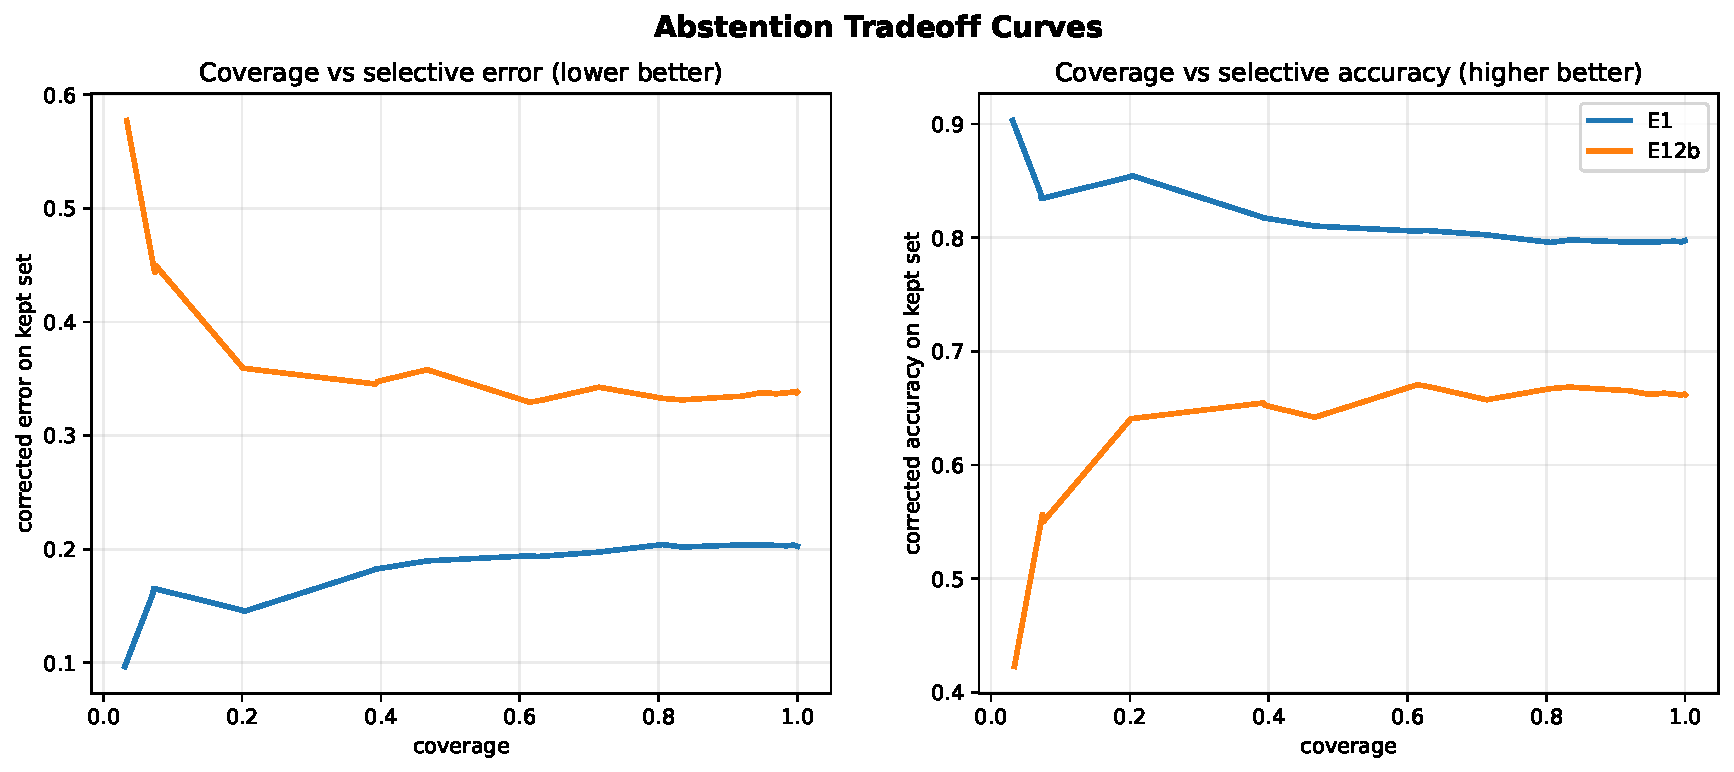
\includegraphics[width=\linewidth]{figures/task7_calibration_report_p4}
  \caption{Abstention trade-off curves. Left: as coverage decreases (more
  abstentions), E1 achieves lower corrected error (reaching $\sim$10\% at
  $5\%$ coverage), while E12b plateaus near 33\%. Right: E1 selective
  accuracy peaks at $\sim$90\% at low coverage, confirming that E1's
  high-confidence corrections are very reliable.}
  \label{fig:abstention_tradeoff}
\end{figure}

\begin{figure}[t]
  \centering
  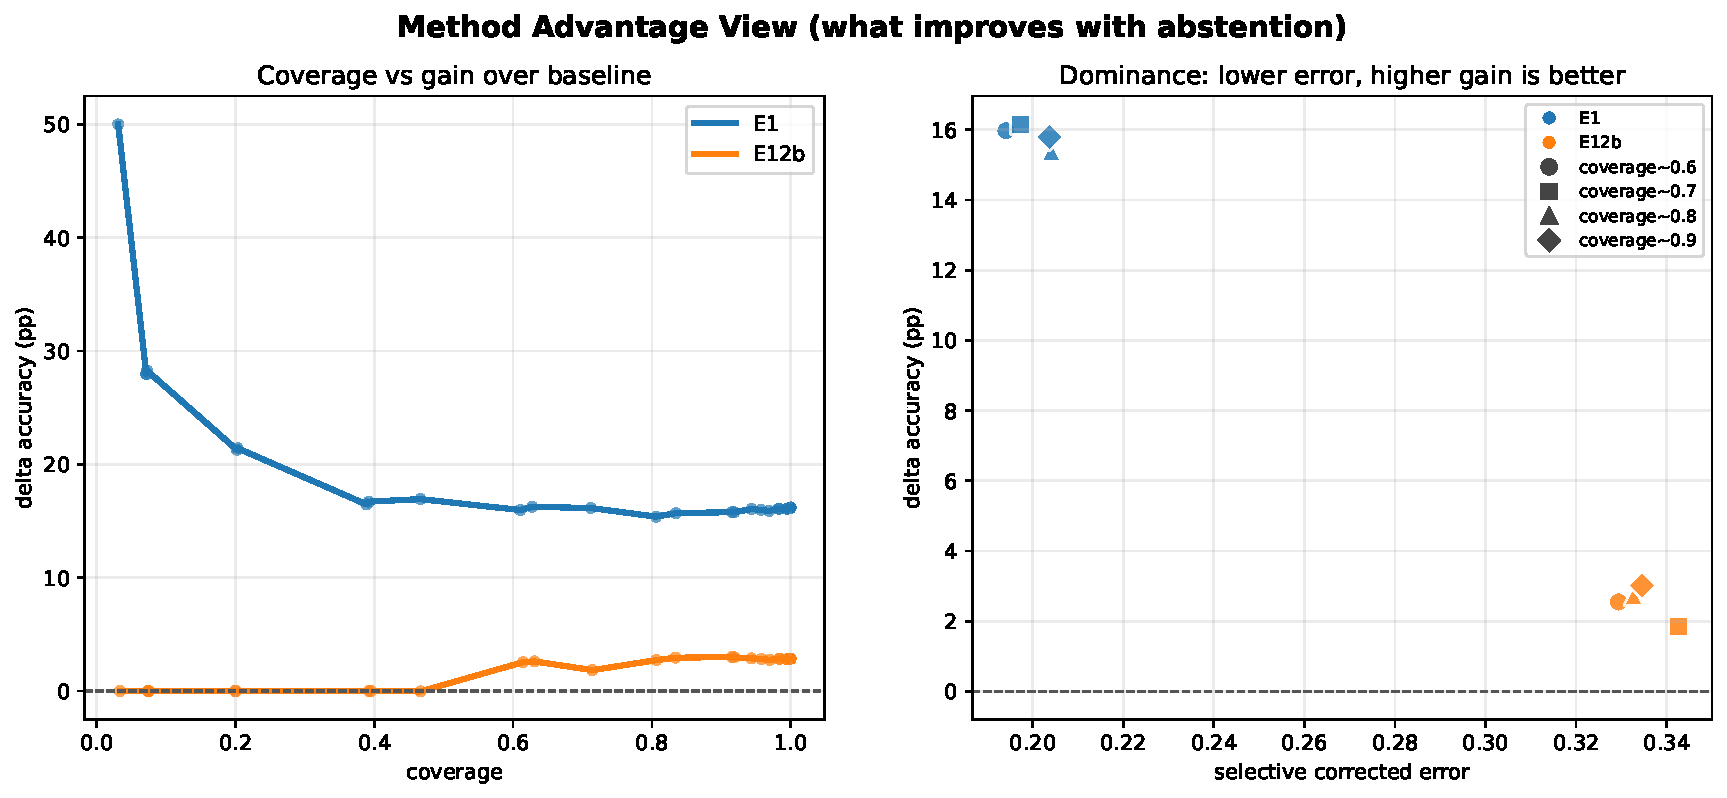
\includegraphics[width=\linewidth]{figures/task7_calibration_report_p5}
  \caption{Left: coverage vs.\ gain over baseline ($\Delta$pp). E1 maintains
  $+16$~pp gain across all coverage levels above 40\%, demonstrating
  broad-coverage robustness. E12b gain varies between 0--3~pp across coverage.
  Right: dominance scatter (error vs.\ gain) at four coverage targets (0.6--0.9);
  E1 operating points cluster tightly near ($0.20$, $+16$~pp), confirming
  stable Pareto dominance over E12b.}
  \label{fig:abstention_gain}
\end{figure}

\begin{figure}[t]
  \centering
  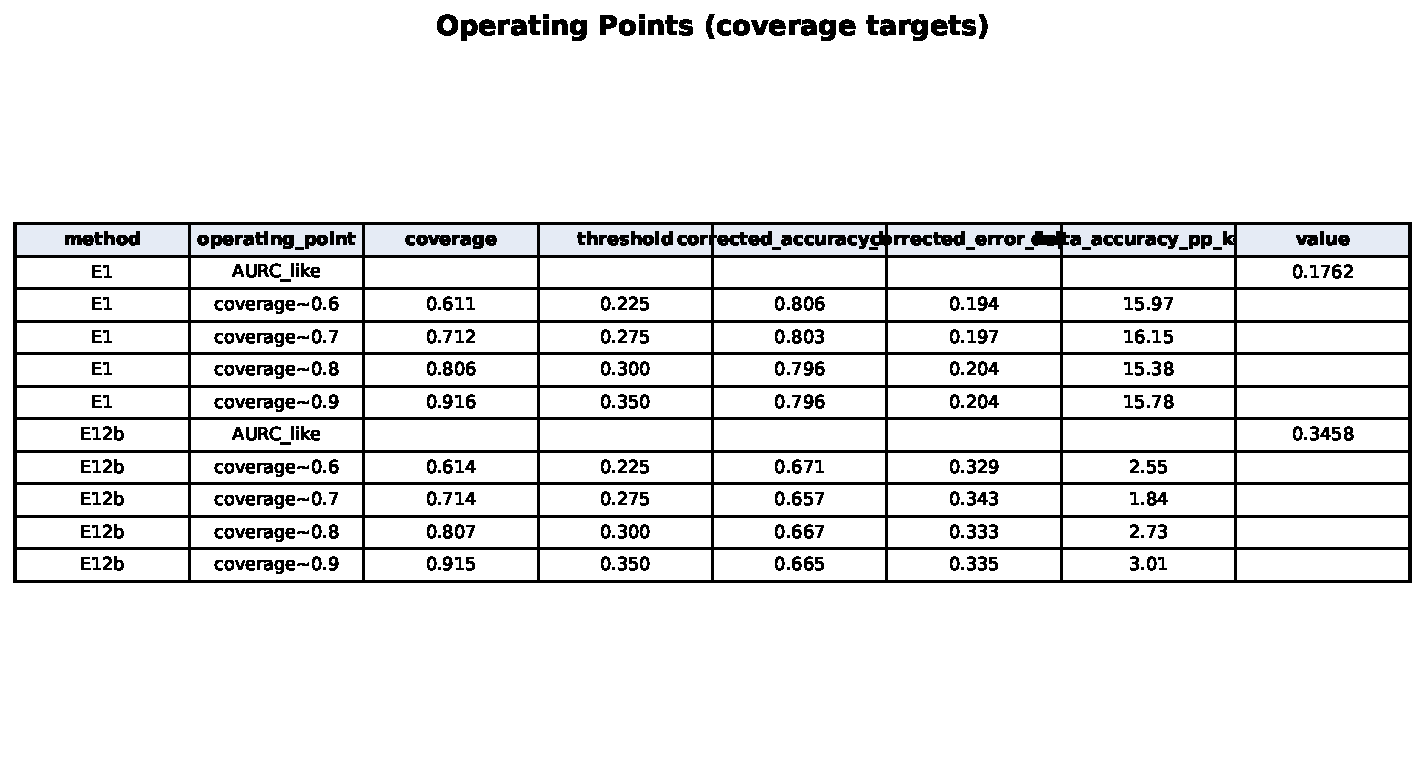
\includegraphics[width=\linewidth]{figures/task7_calibration_report_p7}
  \caption{Operating points table (coverage targets 0.6--0.9). At 60\%
  coverage ($\tau{=}0.225$), E1 achieves 80.6\% selective accuracy
  ($+16.0$~pp over baseline); at 90\% coverage ($\tau{=}0.350$), E1
  maintains 79.6\% ($+15.8$~pp). E12b selective accuracy ranges
  from 65.7\%--67.1\% across the same thresholds, confirming that
  even selective E12b cannot close the gap to E1.}
  \label{fig:abstention_oppoints}
\end{figure}
